\chapter{Experiments and Results}

\section{Classifier Models}

\section{Support Vector Machine Model}
For the spport vector machine model, the kernel was fixed to linear considering the nature of the dataset, which suggests linear separability of driving styles. The focus was on the tuning
of the hyperparameters, such as the regularization parameter $C$, which controls the trade off between achienving a low training error and a low testing error. 
A range of $C$ values were tested to find the optimal value. The model was trained using the \textbf{GridSearchCV} method from the \textbf{sklearn.model\_selection} module.

The best $C$ parameter was identified through cross-validation, optimizing for model accuracy. The best parameters and corresponding score obtained from the grid search were 
accessed via \texttt{svm\_grid.best\_params\_} and \texttt{svm\_grid.best\_score\_}, respectively.

Before proceding to evaluate the model with the balanced and pre-processed dataset, the model was trained using the original dataset to see how it would perform. The accuracy of the model
was evaluated returning a score of 0.88. But then, when running the classification report, it was found that the model was biased towards the majority class as shown in 
Table \ref{table:svm_classification_report}.
It is shown that the model was able to predict the majority class with a precision of 0.88 and a recall of 1.00, but the minority class was not predicted at all. This is a clear 
indication of the model bias towards the majority class, this is due to the imbalanced nature of the dataset.

\begin{table}[H]
    \centering
    \begin{tabular}{|l|l|l|l|l|}
    \hline
    \textbf{Class} & \textbf{Precision} & \textbf{Recall} & \textbf{F1-score} & \textbf{Support} \\ \hline
    AggressiveStyle & 0.00 & 0.00 & 0.00 & 538 \\ \hline
    EvenPaceStyle & 0.89 & 1.00 & 0.94 & 4217 \\ \hline
    \textbf{Accuracy} & \multicolumn{4}{c|}{0.89} \\ \hline
    \textbf{Macro Avg} & 0.44 & 0.50 & 0.47 & 4755 \\ \hline
    \textbf{Weighted Avg} & 0.79 & 0.89 & 0.83 & 4755 \\ \hline
    \end{tabular}
    \caption{Classification Report}
    \label{table:svm_classification_report}
\end{table}

\begin{table}[H]
    \centering
    \begin{tabular}{|c|c|c|}
    \hline
    \multicolumn{3}{|c|}{\textbf{Confusion Matrix}} \\
    \hline
    \textbf{Actual/Predicted} & \textbf{AggressiveStyle} & \textbf{EvenPaceStyle} \\ \hline
    \textbf{AggressiveStyle} & 0 & 538 \\ \hline
    \textbf{EvenPaceStyle} & 0 & 4217 \\ \hline
    \end{tabular}
    \caption{Confusion Matrix}
    \label{table:confusion_matrix}
\end{table}

To resolve the issue of imbalanced dataset that was observed in the SVM model, the use of other techniques such as over-sampling and under-sampling was considered.
SMOTE (Syntetic Minority Over-sampling) which is a statistical technique for increasing the number of instances in the minority class was used. SMOTE works by selecting
examples that are close in the feature space, drawing a line between the examples in the feature space and drawing a new sample at a point along that line. 
It does have some limitations, such as the generation of noisy samples, but it is a widely used technique for dealing with imbalanced datasets. \cite{fernandez2018smote} 
Table \ref{table:classification_report_smote} shows that the application of SMOTE improved the models ability to predict the minority class, which was not predicted at all 
in the previous model. There seems to be be a trade-off; as recall increased, precision decreased. This is expected as the model is now predicting more instances of the minority class.
The F1-score is more balanced, as it is now giving equal weight to both classes. This suggests that while accuracy is lower, the model is now more fair and balanced in its predictions.

\begin{table}[H]
    \centering    
    \begin{tabular}{|l|l|l|l|l|}
    \hline
    \textbf{Class} & \textbf{Precision} & \textbf{Recall} & \textbf{F1-score} & \textbf{Support} \\ \hline
    AggressiveStyle & 0.23 & 0.79 & 0.36 & 538 \\ \hline
    EvenPaceStyle & 0.96 & 0.67 & 0.79 & 4217 \\ \hline
    \textbf{Accuracy} & \multicolumn{4}{c|}{0.68} \\ \hline
    \textbf{Macro Avg} & 0.60 & 0.73 & 0.58 & 4755 \\ \hline
    \textbf{Weighted Avg} & 0.88 & 0.68 & 0.74 & 4755 \\ \hline
    \end{tabular}
    \caption{Classification Report}
    \label{table:classification_report_smote}
\end{table}

% Confusion Matrix
\begin{table}[H]
    \centering
    \begin{tabular}{|c|c|c|}
    \hline
    \multicolumn{3}{|c|}{\textbf{Confusion Matrix}} \\
    \hline
    \textbf{Actual/Predicted} & \textbf{AggressiveStyle} & \textbf{EvenPaceStyle} \\ \hline
    \textbf{AggressiveStyle} & 427 & 111 \\ \hline
    \textbf{EvenPaceStyle} & 1398 & 2819 \\ \hline
    \end{tabular}
    \caption{Confusion Matrix}
    \label{table:confusion_matrix_smote}
\end{table}

\section{Linear Regression Model}
Now with the knowledge about the imbalanced dataset, the new dataset processed with SMOTE was used to train the linear regression model. To find the best parameters for the model,
the \textbf{GridSearchCV} method was used to find the best parameters for the model. The results from \textbf{GridSearchCV} indicated that the best parameter for \textbf{C} was 1000,
which was used to train the model. The model was then evaluated using the balanced dataset and the results are shown in Table \ref{table:log_classification_report} 
and Table \ref{table:log_confusion_matrix}.


\begin{table}[H]
    \centering    
    \begin{tabular}{|l|l|l|l|l|}
    \hline
    \textbf{Class} & \textbf{Precision} & \textbf{Recall} & \textbf{F1-score} & \textbf{Support} \\ \hline
    AggressiveStyle & 0.24 & 0.75 & 0.37 & 538 \\ \hline
    EvenPaceStyle & 0.96 & 0.70 & 0.81 & 4217 \\ \hline
    \textbf{Accuracy} & \multicolumn{4}{c|}{0.71} \\ \hline
    \textbf{Macro Avg} & 0.60 & 0.73 & 0.59 & 4755 \\ \hline
    \textbf{Weighted Avg} & 0.88 & 0.71 & 0.76 & 4755 \\ \hline
    \end{tabular}
    \caption{Classification Report for Logistic Regression}
    \label{table:log_classification_report}
\end{table}

% Confusion Matrix for Logistic Regression
\begin{table}[H]
    \centering
    \begin{tabular}{|c|c|c|}
    \hline
    \multicolumn{3}{|c|}{\textbf{Confusion Matrix for Logistic Regression}} \\
    \hline
    \textbf{Actual/Predicted} & \textbf{AggressiveStyle} & \textbf{EvenPaceStyle} \\ \hline
    \textbf{AggressiveStyle} & 404 & 134 \\ \hline
    \textbf{EvenPaceStyle} & 1268 & 2949 \\ \hline
    \end{tabular}
    \caption{Confusion Matrix for Logistic Regression}
    \label{table:log_confusion_matrix}
\end{table}

After optimizing the model parameters and evaluating its predictive performance, it is important to understand which features contribute most significantly to the model's predictions. 
In logistic regression, the coefficients associated with each feature can indicate the importance and influence of that feature on the model's output. 

To visualize the impact of each feature, a coefficient plot can be constructed. This plot ranks the features by their coefficients, providing clear insights into which features are 
most informative for predicting the target variable.

\begin{figure}[H]
    \centering
    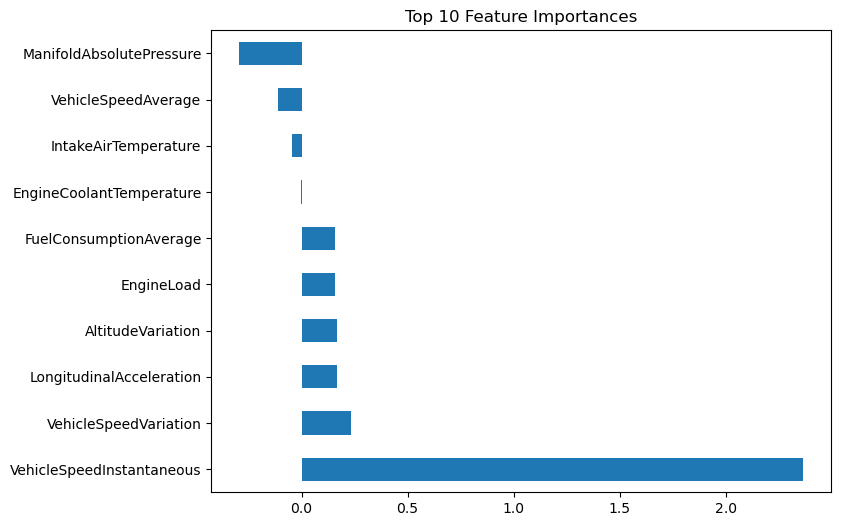
\includegraphics[width=0.9\textwidth]{images/feature_importance.png} 
    \caption{Top 10 Feature Importances in the Logistic Regression Model}
    \label{fig:feature_importances}
\end{figure}

This coefficient plot shows the relative importance of features in predicting driving styles. Features with larger absolute values of coefficients have a greater impact on the model's 
decision-making process. It is a good way to understand which features are most important for the model's predictions. The top 10 features are shown in Figure ~\ref{fig:feature_importances}.

\section{K-Nearest Neighbors Model}
The k-Nearest Neighbors (kNN) model was trained using the balanced dataset and the results are shown in Table \ref{table:knn_classification_report} and Table \ref{table:knn_confusion_matrix}.
The kNN model was able to predict the minority class with a precision of 0.59 and a recall of 0.81. The model was able to predict the majority class with a precision of 0.97
and a recall of 0.93. The accuracy of the model was 0.92, which is higher than the previous models. The F1-score is also higher than the previous models, suggesting that the model
is more balanced in its predictions.

\begin{table}[H]
    \centering    
    \begin{tabular}{|l|l|l|l|l|}
    \hline
    \textbf{Class} & \textbf{Precision} & \textbf{Recall} & \textbf{F1-score} & \textbf{Support} \\ \hline
    AggressiveStyle & 0.59 & 0.81 & 0.68 & 538 \\ \hline
    EvenPaceStyle & 0.97 & 0.93 & 0.95 & 4217 \\ \hline
    \textbf{Accuracy} & \multicolumn{4}{c|}{0.92} \\ \hline
    \textbf{Macro Avg} & 0.78 & 0.87 & 0.82 & 4755 \\ \hline
    \textbf{Weighted Avg} & 0.93 & 0.92 & 0.92 & 4755 \\ \hline
    \end{tabular}
    \caption{Classification Report for k-Nearest Neighbors (kNN)}
    \label{table:knn_classification_report}
\end{table}


\begin{table}[H]
    \centering
    \begin{tabular}{|c|c|c|}
    \hline
    \multicolumn{3}{|c|}{\textbf{Confusion Matrix for k-Nearest Neighbors (kNN)}} \\
    \hline
    \textbf{Actual/Predicted} & \textbf{AggressiveStyle} & \textbf{EvenPaceStyle} \\ \hline
    \textbf{AggressiveStyle} & 436 & 102 \\ \hline
    \textbf{EvenPaceStyle} & 299 & 3918 \\ \hline
    \end{tabular}
    \caption{Confusion Matrix for k-Nearest Neighbors (kNN)}
    \label{table:knn_confusion_matrix}
\end{table}



\section{Results}

The Support Vector Machine (SVM) model, initially trained on the imbalanced dataset, improved after the dataset was balanced using SMOTE, achieving 0.88 accuracy. Linear Regression,
opmized with GridSearchCV, achieved 0.71 accuracy with feature importance analysis as shown in Figure \ref{fig:feature_importances}. The k-Nearest Neighbors (kNN) model outperformed,
achieving 0.92 accuracy, effectively predicting both classes. Results demonstrate that the kNN model is the best model for this dataset, with the highest accuracy and F1-score. 
Linear regression and SVM models are not as effective in predicting the minority class.

